\chapter{Кратчайшие}
\label{chap:shortest}

\section{Внутренняя геометрия}

Геометрию поверхностей разделяют на внутреннюю и внешнюю.
\index{внутренняя геометрия}\emph{Внутренним} называется всё, что можно проверить или померить не вылазя из поверхности,
как например, углы между кривыми на поверхности или длины этих.
В противном случае, если в определении существенно использует объемлющее пространство, то мы определяем что-то \index{внешняя геометрия}\emph{внешнее};
нормальная кривизна тому пример.

Средняя кривизна, как и гауссова, определяются через главные кривизны, которые являются внешними.
Позднее (\ref{thm:remarkable}) будет показано, что гауссова кривизна является внутренней, то есть её таки можно найти при помощи измерений на самой поверхности.
Средняя же кривизна не является внутренней; например, внутренняя геометрия плоскости не отличается от внутренней геометрии графика $z\z=(x+y)^2$.
Однако, средняя кривизна первой поверхности равна нулю во всех точках, в то время как средняя кривизна второй не равна нулю, например, в начале координат.

Следующее упражнение поможет настроиться на нужный лад;
оно может показаться нудной задачей по анализу, но на самом деле это забавная задача по геометрии.

\begin{wrapfigure}[7]{r}{33 mm}
\vskip-0mm
\centering
\includegraphics{mppics/pic-77}
\vskip-0mm
\end{wrapfigure}

\begin{thm}{Упражнение}\label{ex:lasso}
Ковбой стоит у подножия ледяной горы, в виде конуса с круглым основанием и углом наклона~$\theta$.
Он забрасывает лассо на вершину конуса, затягивает его и пытается подняться.

Найти максимальный угол $\theta$, при котором ковбой не может забраться на гору.
\end{thm}


\section{Определение}

Пусть $p$ и $q$ --- точки на поверхности~$\Sigma$.
Напомним, что $\dist{p}{q}\Sigma$ обозначает внутреннее расстояние от $p$ до~$q$;
то есть это наименьшая верхняя грань длин путей на $\Sigma$ из $p$ в~$q$.

Путь $\gamma$ из $p$ в $q$ на $\Sigma$, минимизирующий длину, называется \index{кратчайшая}\emph{кратчайшей} из $p$ в~$q$.
Образ такой кратчайшей будет обозначаться $[p,q]$ или $[p,q]_\Sigma$.\index{10aac@$[p,q]$, $[p,q]_\Sigma$ (кратчайшая)}
Если мы пишем $[p,q]_\Sigma$, то считается, что кратчайшая существует, и мы выбрали одну из них.
Вообще говоря, такие кратчайшие не обязаны существовать, или же их может быть больше одной;
это показано в следующих двух примерах.

\begin{wrapfigure}[9]{r}{28 mm}
\vskip-6mm
\centering
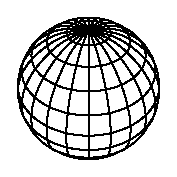
\includegraphics{asy/sphere}
\bigskip
\includegraphics{mppics/pic-79}
\end{wrapfigure}

\parbf{Неединственность.}
Между полюсами сферы каждый меридиан --- кратчайшая.
Это следует из \ref{obs:S2-length}.

\parbf{Несуществование.}
Пусть $\Sigma$ --- плоскость $(x,y)$ с удалённым началом координат.
Рассмотрим на ней две точки $p=(1,0,0)$ и $q\z=(-1,0,0)$.
Покажем, что \textit{на~$\Sigma$ нету кратчайших из $p$ в $q$.}

Заметим, что $\dist{p}{q}\Sigma=2$. 
Действительно, пусть $s_\epsilon=(0,\epsilon,0)$ при $\epsilon\z>0$.
Ломаная $ps_\epsilon q$ лежит на $\Sigma$;
её длина $2\cdot\sqrt{1+\epsilon^2}$ стремится к 2 при $\epsilon\to0$.
Отсюда $\dist{p}{q}\Sigma\le 2$.
А поскольку $\dist{p}{q}\Sigma\z\ge \dist{p}{q}{\mathbb{R}^3}=2$, получаем, что $\dist{p}{q}\Sigma=2$.

Следовательно, кратчайшая из $p$ в $q$, если она существует, должна иметь длину~2.
По неравенству треугольника, любая кривая длины 2 из $p$ в $q$ обязана идти вдоль отрезка $[p,q]$;
и в частности, содержать начало координат.
Ну а поскольку в $\Sigma$ нету начала координат, то ней нету и кратчайшей из $p$ в $q$. 

\begin{thm}{Предложение}\label{prop:shortest-paths-exist}
Любые две точки на собственной гладкой поверхности (возможно, с краем) соединимы кратчайшей.
\end{thm}

\parbf{Доказательство.}
Пусть $p$ и $q$ --- точки на собственной гладкой поверхности~$\Sigma$, и $\ell=\dist{p}{q}\Sigma$.

Поскольку $\Sigma$ гладкая, точки $p$ и $q$ соединимы в $\Sigma$ кусочно-гладким путём.
Любой такой путь спрямляем, а значит, $\ell\z<\infty$.

По определению индуцированной внутренней метрики (\ref{sec:Length metric})
на $\Sigma$ существует последовательность путей $\gamma_n$ из $p$ в $q$, таких что
\[\length\gamma_n\to \ell\quad\text{при}\quad n\to \infty.\]

Можно считать, что $\length\gamma_n<\ell+1$ для любого $n$, и каждый $\gamma_n$ параметризован пропорционально длине его дуги.
В частности, каждый путь $\gamma_n\:[0,1]\to\Sigma$ липшицев с константой $(\ell+1)$; 
то есть
\[|\gamma(t_0)-\gamma(t_1)|\le (\ell+1)\cdot|t_0-t_1|\]
для любых $t_0,t_1\in[0,1]$.

При любом $n$, образ $\gamma_n$ лежит в замкнутом шаре $\bar B[p,\ell+1]$.
Следовательно, координатные функции всех $\gamma_n$ равномерно непрерывны и ограничены.
По теореме Арцела --- Асколи (\ref{lem:equicontinuous}),
существует сходящаяся подпоследовательность $\gamma_n$, и её предел, скажем $\gamma_\infty\:[0,1]\to\mathbb{R}^3$, непрерывен;
то есть это путь.
Кривая $\gamma_\infty$ идёт из $p$ в $q$,
и в частности,
\[\length\gamma_\infty\ge \ell.\]
Поскольку $\Sigma$ --- замкнутое множество, $\gamma_\infty$ лежит в~$\Sigma$.

По полунепрерывности длины (\ref{thm:length-semicont}), $\length\gamma_\infty\le \ell$.
Следовательно, $\length\gamma_\infty\z= \ell$, и $\gamma_\infty$ --- кратчайшая из $p$ в~$q$.
\qeds


\section{Короткая проекция}

Следующая лемма относится к выпуклой геометрии,
но будет играть столь важную роль, что мы её докажем.

\begin{thm}{Лемма}\label{lem:nearest-point-projection}
Пусть $R$ --- замкнутое выпуклое множество в $\mathbb{R}^3$.
Для любой точки $p\in\mathbb{R}^3$ существует единственная точка $\bar p\z\in R$, которая минимизирует расстояние до $R$;
то есть $|p-\bar p|\le |p-x|$ для любой точки $x\in R$.

Более того, отображение $p\mapsto \bar p$ короткое;
то есть
\[|p-q|\ge|\bar p-\bar q| \eqlbl{eq:short-cpp}\]
для любой пары точек $p,q\in \mathbb{R}^3$.
\end{thm}

Отображение $p\mapsto \bar p$ будет называться \label{проекция на ближайшую точку}\index{короткая проекция}\emph{короткой проекцией};
оно отображает евклидово пространство в~$R$.
Отметим, что $\bar p=p$ для любой точки $p\in R$.
В частности, $\bar{\bar p}\equiv\bar p$.

\parbf{Доказательство.}
Выберем $p\in \mathbb{R}^3$.
Пусть 
\[\ell=\inf\set{|p-x|}{x\in R},\]
и $x_n\in R$ такая последовательность, что $|p-x_n|\to \ell$ при $n\to\infty$.

Не умаляя общности, можно считать, что все точки $x_n$ лежат в шаре радиуса $\ell+1$ с центром в~$p$.
Значит, у последовательности $x_n$ найдётся \index{частичный предел}\emph{частичный предел}, скажем $\bar p$;
то есть $\bar p$ --- предел некоторой подпоследовательности $x_n$.
Множество $R$ замкнуто, и, значит, $\bar p\in R$.
По построению 
\begin{align*}
|p-\bar p|&=\lim_{n\to\infty}|p-x_n|=\ell,
\end{align*}
и существование доказано.

{

\begin{wrapfigure}{l}{22 mm}
\vskip-0mm
\centering
\includegraphics{mppics/pic-40}
\vskip-0mm
\end{wrapfigure}

Допустим, что существуют две различные точки $\bar p, \bar p'\in R$, минимизирующие расстояние до~$p$.
Так как $R$ выпукло, их середина $m=\tfrac12\cdot (\bar p+\bar p')$ лежит в~$R$.
Заметим, что $|p-\bar p|\z=|p-\bar p'|=\ell$;
то есть $[p\bar p\bar p']$ --- равнобедренный треугольник.
Следовательно, $[p\bar p m]$ --- прямоугольный треугольник.
Поскольку катет короче гипотенузы, $|p-m|<\ell$ --- противоречие. 

Остаётся проверить \ref{eq:short-cpp}.
Можно считать, что $\bar p\ne\bar q$; иначе и доказывать нечего.

}

Если $\measuredangle \hinge{\bar p}{p}{\bar q}< \tfrac\pi2$, то $\dist{p}{x}{}\z<\dist{p}{\bar p}{}$ для точки $x\in [\bar p,\bar q]$, близкой к $\bar p$,
а это невозможно поскольку $[\bar p,\bar q]\subset K$.

{

\begin{wrapfigure}{r}{37 mm}
\vskip-8mm
\centering
\includegraphics{mppics/pic-41}
\vskip-0mm
\end{wrapfigure}

Значит $\measuredangle \hinge{\bar p}{p}{\bar q}\ge \tfrac\pi2$ или же $p=\bar p$.
В обоих случаях ортогональная проекция $p$ на прямую $\bar p\bar q$ лежит до $\bar p$ или совпадает с $\bar p$.
Аналогично доказывается, что проекция $q$ на прямую $\bar p\bar q$ лежит после $\bar q$ или совпадает с~$\bar q$.
Значит, проекция $[p,q]$ содержит $[\bar p,\bar q]$,
и \ref{eq:short-cpp} следует.
\qeds

}

\section{Кратчайшие на выпуклых поверхностях}

\begin{thm}{Теорема}\label{thm:shorts+convex}
Предположим, что поверхность $\Sigma$ ограничивает замкнутую выпуклую область $R$, и $p,q\in \Sigma$.
Обозначим через $W$ внешнюю замкнутую область $\Sigma$;
то есть $W$ включает $\Sigma$ и дополнение к~$R$.
Тогда 
\[\length\gamma\ge \dist{p}{q}\Sigma\]
для любого пути $\gamma$ в $W$ от $p$ до~$q$.
Более того, если $\gamma$ не лежит в $\Sigma$, то неравенство строгое.
\end{thm}

\parbf{Доказательство.}
Пусть $\bar\gamma$ --- короткая проекция $\gamma$ на $R$.
Кривая $\bar\gamma$ идёт по $\Sigma$ из $p$ в $q$; следовательно, 
\[\length\bar\gamma\ge \dist{p}{q}\Sigma.\]

Давайте покажем, что 
\[\length\gamma\ge\length\bar\gamma.
\eqlbl{bar-gamma=<gamma}\]
Рассмотрим ломаную $\bar p_0\dots \bar p_n$, вписанную в $\bar\gamma$.
Пусть $p_0\dots p_n$ --- соответствующая ломаная, вписанная в $\gamma$;
то есть $p_i=\gamma(t_i)$, если $\bar p_i\z=\bar\gamma(t_i)$.
Согласно \ref{lem:nearest-point-projection}, $|p_i-p_{i-1}|\z\ge|\bar p_i-\bar p_{i-1}|$ для любого~$i$.
Следовательно,
\[\length p_0\dots p_n\ge \length \bar p_0\dots \bar p_n.\]
Применив определение длины, получаем \ref{bar-gamma=<gamma}, и первое утверждение следует;
осталось второе.

\begin{wrapfigure}{o}{37 mm}
\vskip-0mm
\centering
\includegraphics{mppics/pic-82}
\vskip-0mm
\end{wrapfigure}

Допустим, что существует точка $w\z=\gamma(t_1)\z\notin\Sigma$;
заметим, что $w\notin R$.
Тогда существует плоскость $\Pi$, отделяющая $w$ от~$\Sigma$ (см.~\ref{lem:separation}).

Кривая $\gamma$ должна пересечь $\Pi$ в паре точек, до и после $t_1$.
Пусть $a=\gamma(t_0)$ и $b=\gamma(t_2)$ --- эти точки.
Дуга $\gamma$ от $a$ до $b$ длиннее, чем $|a-b|$,
ведь её длина не меньше $|a-w|+|w-b|$, а $|a-w|\z+|w-b|>|a-b|$, так как $w\notin[a,b]$.

Заменим в $\gamma$ дугу от $a$ до $b$ на отрезок $[a,b]$.
Обозначим полученную кривую через $\gamma_1$, тогда
\[\length\gamma>\length \gamma_1.\]

Из выше сказанного,
\[\length \gamma_1\ge \dist{p}{q}\Sigma,\]
ибо $\gamma_1$ лежит в~$W$.
И второе утверждение следует.
\qeds

\begin{thm}{Упражнение}\label{ex:length-dist-conv}
Пусть $\Sigma$ --- открытая или замкнутая гладкая поверхность с положительной гауссовой кривизной, и $\Norm$ --- её поле нормалей.
Покажите, что 
\[\dist{p}{q}\Sigma\le 2\cdot \frac{|p-q|}{|\Norm(p)+\Norm(q)|}\]
для любых $p,q\in \Sigma$.
\end{thm}


\begin{wrapfigure}{r}{27 mm}
\vskip-14mm
\centering
\includegraphics{mppics/pic-240}
\end{wrapfigure}

\begin{thm}{Упражнение}\label{ex:hat-convex}
Пусть плоскость $\Pi$ отсекает горбушку $\Delta$ от замкнутой гладкой поверхности~$\Sigma$.
Предположим, что $\Sigma$ ограничивает выпуклую область $R$, и отражение внутренней части $\Delta$ в $\Pi$ лежит внутри $R$.
Покажите, что $\Delta$ является \index{выпуклое множество}\emph{выпуклой} по внутренней метрике $\Sigma$;
то есть 
если оба конца кратчайшей в $\Sigma$ 
лежат в $\Delta$,
то и вся она лежит в $\Delta$.
\end{thm}

Определим \index{внутренний диаметр}\emph{внутренний диаметр} поверхности как точную верхнюю грань длин кратчайших на ней.

\begin{thm}{Упражнение}\label{ex:intrinsic-diameter}
Пусть $\Sigma$ --- замкнутая гладкая поверхность с положительной гауссовой кривизной, лежащая в единичном шаре.

\begin{subthm}{}
Покажите, что внутренний диаметр $\Sigma$ не превышает~$\pi$.
\end{subthm}

\begin{subthm}{}
Покажите, что площадь $\Sigma$ не может превышать $4\cdot \pi$.
\end{subthm}

\end{thm}
